这里,我们希望下面的函数是协程:

\begin{cpp}
void coro(int max)
{
	std::cout << "CORO " << max << " start\n";

	for (int val = 1; val <= max; ++val) {
		std::cout << "CORO " << val << '/' << max << '\n';
	}

	std::cout << "CORO " << max << " end\n";
}
\end{cpp}

该函数有一个表示最大值的形参,首先将其打印出来。然后,从1循环到这个最大值,并打印每个值,最后有一个print语句。

当用coro(3)调用该函数时,有以下输出:

\begin{shell}
CORO 3 start
CORO 1/3
CORO 2/3
CORO 3/3
CORO 3 end
\end{shell}

但是,我们希望将其编程为一个协程,每次执行循环中的print语句时,都会挂起。因此,函数可中断,协程的用户可以通过恢复触发下一个值的输出。

\mySubsubsection{14.2.1}{定义协程}

以下是协程定义的完整代码:

\filename{coro/coro.hpp}

\begin{cpp}
#include <iostream>
#include "corotask.hpp" // for CoroTask

CoroTask coro(int max)
{
	std::cout << "             CORO " << max << " start\n";

	for (int val = 1; val <= max; ++val) {
		// print next value:
		std::cout << "          CORO " << val << '/' << max << '\n';

		co_await std::suspend_always{}; // SUSPEND
	}

	std::cout << " CORO " << max << " end\n";
}
\end{cpp}

仍然有一种循环遍历这些值直到参数max的函数,但有两点与普通函数不同:

\begin{itemize}
\item
print语句后的循环中,有一个co\_await表达式,其可挂起协程并阻塞它,直到协程恢复,这称为挂起点。

挂起调用的确切行为由紧跟在co\_await后面的表达式定义,使开发者能够控制挂起的确切行为。

目前,将使用std::suspend\_always类型的默认构造对象,其接受挂起并将控制权交还给调用者。也可以通过将特殊操作数传递给co\_await,来拒绝挂起或恢复另一个协程。

\item
虽然协程没有返回语句,但其有一个返回类型CoroTask。此类型用作协程调用者的协程接口,但不能将返回类型声明为auto。

返回类型是必需的,因为调用者需要一个接口来处理协程(例如恢复它)。C++20中,协程接口类型必须由程序员(或第三方库)提供,稍后将看到是如何实现的。计划是,即将到来的C++标准将在其库中提供一些标准的协程接口类型。
\end{itemize}

\mySubsubsection{14.2.2}{使用协程}

可以这样使用协程:

\filename{coro/coro.cpp}

\begin{cpp}
#include <iostream>
#include "coro.hpp"

int main()
{
	// start coroutine:
	auto coroTask = coro(3); // initialize coroutine
	std::cout << "coro() started\n";

	// loop to resume the coroutine until it is done:
	while (coroTask.resume()) { // RESUME
		std::cout << "coro() suspended\n";
	}

	std::cout << "coro() done\n";
}
\end{cpp}

初始化协程后,产生协程接口coroTask,启动一个循环,在协程挂起后,一次又一次地恢复协程:

\begin{cpp}
auto coroTask = coro(3); // initialize coroutine

while (coroTask.resume()) { // RESUME
	...
}
\end{cpp}

通过调用coro(3),像调用函数一样调用协程。然而,与函数调用相比,不等待协程结束。相反,在协程初始化之后,调用返回协程接口来处理协程(在开始处有一个隐式挂起点)。

在这里使用auto作为协程接口类型,也可以使用它的类型,这是协程的返回类型:

\begin{cpp}
CoroTask coroTask = coro(3); // initialize coroutine
\end{cpp}

类CoroTask提供的API提供了一个成员函数resume(),可用于恢复协程。每次调用resume()都允许协程继续运行,直到下一次挂起或直到协程结束。请注意,挂起不会在协程中留下任何作用域。在恢复时,可继续暂停状态下的协程。

其效果是,在main()的循环中,调用协程中的下一组语句,直到挂起点或结束:

\begin{itemize}
\item
首先,初始输出,val的初始化,以及循环中的第一个输出:

\begin{cpp}
std::cout << "                 CORO " << max << " start\n";
for (int val = 1; val <= max; ... ) {
	std::cout << "               CORO " << val << '/' << max << '\n';
	...
}
\end{cpp}

\item
然后是两次,循环中的下一个迭代:

\begin{cpp}
	for (...; val <= max; ++val) {
		std::cout << "               CORO " << val << '/' << max << '\n';
		...
	}
\end{cpp}

\item
最后,在循环中的最后一次迭代之后,协程执行最后的print语句:

\begin{cpp}
for ( ... ; val <= max; ++val) {
	...
}

std::cout << " CORO " << max << " end\n";
\end{cpp}
\end{itemize}

程序输出如下所示:

\begin{shell}
coro() started
         CORO 3 start
         CORO 1/3
coro() suspended
         CORO 2/3
coro() suspended
         CORO 3/3
coro() suspended
         CORO 3 end
coro() done
\end{shell}


\begin{center}
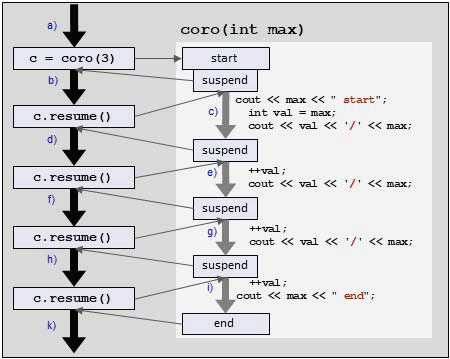
\includegraphics[width=0.6\textwidth]{content/chapter14/images/2.png}\\
图14.2 协同程序的例子
\end{center}

结合接口类型CoroTask,我们马上就会看到,可得到以下控制流(见图14.2):

\begin{enumerate}[label=\alph*)]
\item
首先,调用协程,使其启动。协程立即挂起,调用返回处理协程的接口对象。

\item
然后,可以使用接口对象来恢复协程,以便执行其语句。

\item
协程内部,处理开始语句直到第一个挂起点:第一个print语句,在循环头部初始化局部计数器val,以及(在检查val小于或等于max之后)循环内的print语句。在这部分结束时,协程暂停。

\item
挂起将控制转移回主函数,然后主函数继续执行,直到再次恢复协程。

\item
协程继续执行下一个语句,直到再次到达挂起点,增加val并(在检查val仍然小于或等于max之后)在循环中执行print语句。在这部分结束时,协程再次挂起。

这里继续使用之前协程挂起时val的值。

\item
再次将控制转移回主函数,然后主函数继续运行,直到再次恢复协程。

\item
只要增量val小于或等于max,协程就继续循环。

\item
只要协程co\_await挂起,主函数就会恢复协程。

\item
最后,协程在val加1之后离开循环,调用最后的print语句,值为max。

\item
协程结束时,最后一次将控制转回主函数。然后main函数结束循环,并继续运行直到结束。
\end{enumerate}

协程的初始化和接口的确切行为取决于接口类型CoroTask,可能只是启动协程或提供具有一些初始化的上下文,例如打开文件或启动线程,还定义协程是立即启动还是惰性启动(立即挂起)。在CoroTask的当前实现中,是惰性启动的,所以协程的初始调用还没有执行coro()。

这里没有异步通信或控制流,coroTask.resume()更像是coro()下一部分的函数调用。

当到达协程的末尾时,循环结束,resume()的实现使得它返回协程是否(尚未)完成。当resume()返回true时,继续循环(在打印暂停之后)。

\mySamllsection{多次使用协程}

协程是一种准并行函数,通过来回切换控制流来顺序执行。其状态存储在由协程句柄控制的堆内存中,该句柄通常由协程接口持有。通过拥有多个协程接口对象,可以处理多个活动协程的状态,这些协程可能彼此独立地运行或挂起。

假设用不同的max值启动两个协程:

\filename{coro/coro2.cpp}

\begin{cpp}
#include <iostream>
#include "coro.hpp"

int main()
{
	// start two coroutines:
	auto coroTask1 = coro(3); // initialize 1st coroutine
	auto coroTask2 = coro(5); // initialize 2nd coroutine
	std::cout << "coro(3) and coro(5) started\n";

	coroTask2.resume(); // RESUME 2nd coroutine once

	// loop to resume the 1st coroutine until it is done:
	while (coroTask1.resume()) { // RESUME 1st coroutine
		std::cout << "coro() suspended\n";
	}

	std::cout << "coro() done\n";

	coroTask2.resume(); // RESUME 2nd coroutine again
}
\end{cpp}

对于初始化的协程,可得到两个不同的接口对象,coroTask1和coroTask2。通过有时恢复第一个协程,有时恢复第二个协程,控制流在主函数和这两个协程之间跳转。

例子中,恢复第二个协程(最大5个)一次,然后循环恢复第一个协程,最后再次恢复第二个协程。结果,程序有以下输出:

\begin{shell}
coro(3) and coro(5) started
         CORO 5 start
         CORO 1/5
         CORO 3 start
         CORO 1/3
coro() suspended
         CORO 2/3
coro() suspended
         CORO 3/3
coro() suspended
         CORO 3 end
coro() done
         CORO 2/5
\end{shell}

甚至可以将协程接口对象传递给不同的函数或线程那里恢复,其将永远保持目前的状态。

\mySubsubsection{14.2.3}{引用调用的生命周期问题}

协程的生命周期通常比最初调用它的语句要长。这有一个重要的后果:若通过引用传递临时对象,可能会遇到致命的运行时问题。

考虑以下稍微修改过的协程,现在所做的就是通过引用,取最大值:

\filename{coro/cororef.hpp}

\begin{cpp}
#include <iostream>
#include <coroutine> // for std::suspend_always{}
#include "corotask.hpp" // for CoroTask

CoroTask coro(const int& max)
{
	std::cout << "   CORO " << max << " start\n"; // OOPS: value of max still valid?

	for (int val = 1; val <= max; ++val) { // OOPS: value of max still valid?
		std::cout << " CORO " << val << '/' << max << '\n';
		co_await std::suspend_always{}; // SUSPEND
	}

	std::cout << " CORO " << max << " end\n"; // OOPS: value of max still valid?
}
\end{cpp}

问题是,传递一个临时对象(甚至可能是一个文字对象)会创建未定义行为。可能会看到它,也可能不会看到它,这取决于平台、编译器设置和其他代码。例如,考虑使用如下方式调用协程:

\filename{coro/cororef.cpp}

\begin{cpp}
#include <iostream>
#include "cororef.hpp"

int main()
{
	auto coroTask = coro(3); // OOPS: creates reference to temporary/literal
	std::cout << "coro(3) started\n";
	coro(375); // another temporary coroutine
	std::cout << "coro(375) started\n";
	// loop to resume the coroutine until it is done:

	while (coroTask.resume()) { // ERROR: undefined behavior
		std::cout << "coro() suspended\n";
	}
	std::cout << "coro() done\n";
}
\end{cpp}

某些平台上,此代码运行良好。然而,在我测试这段代码的一个平台上,得到了以下输出:

\begin{shell}
coro(3) started
coro(375) started
  CORO -2147168984 start
  CORO -2147168984 end
coro() done
\end{shell}

初始化协程的语句之后,max引用所引用的传入参数3的位置不再可用。当第一次恢复协程时,val的输出和初始化使用对已销毁对象的引用。

通常: \textbf{不要使用引用来声明协程参数。}

若复制参数的代价太大,可以通过使用std::ref()或std::cref()创建的引用包装器“按引用传递”。对于容器,可以使用std::views::all(),将容器作为视图传递,因此可以使用所有标准范围函数,而无需将参数转换回来。例如:

\begin{cpp}
CoroTask printElems(auto coll)
{
	for (const auto& elem : coll) {
		std::cout << elem << '\n';
		co_await std::suspend_always{}; // SUSPEND
	}
}
std::vector<std::string> coll;
...
// start coroutine that prints the elements:
// - use view created with std::views::all() to avoid copying the container
auto coPrintElems = printElems(std::views::all(coll));

while (coPrintElems.resume()) { // RESUME
...
}
\end{cpp}

\mySubsubsection{14.2.4}{调用协程}

协程可以调用其他协程(甚至是间接的),调用和被调用的协程都可能有挂起点。

考虑一个具有一个挂起点的协程,以便其分两部分运行:

\begin{cpp}
CoroTask coro()
{
	std::cout << " coro(): PART1\n";
	co_await std::suspend_always{}; // SUSPEND
	std::cout << " coro(): PART2\n";
}
\end{cpp}

这样使用这个协程时:

\begin{cpp}
auto coroTask = coro(); // initialize coroutine
std::cout << "MAIN: coro() initialized\n";

while (coroTask.resume()) { // RESUME
	std::cout << "MAIN: coro() suspended\n";
}

std::cout << "MAIN: coro() done\n";
\end{cpp}

可得到以下输出:

\begin{shell}
MAIN: coro() initialized
    coro(): PART1
MAIN: coro() suspended
    coro(): PART2
MAIN: coro() done
\end{shell}

现在,通过另一个协程间接调用coro()。main()调用callCoro(),而非coro():

\begin{cpp}
auto coroTask = callCoro(); // initialize coroutine
std::cout << "MAIN: callCoro() initialized\n";

while (coroTask.resume()) { // RESUME
	std::cout << "MAIN: callCoro() suspended\n";
}

std::cout << "MAIN: callCoro() done\n";
\end{cpp}

有趣的部分是如何实现callCoro()。

\mySamllsection{无内部resume()}

可以尝试通过coro()来实现callCoro():

\begin{cpp}
CoroTask callCoro()
{
	std::cout << " callCoro(): CALL coro()\n";
	coro(); // CALL sub-coroutine
	std::cout << " callCoro(): coro() done\n";
	co_await std::suspend_always{}; // SUSPEND
	std::cout << " callCoro(): END\n";
}
\end{cpp}

这段代码可编译。然而,并没有像预期的那样工作,正如程序的输出所示:

\begin{shell}
MAIN: callCoro() initialized
  callCoro(): CALL coro()
  callCoro(): coro() done
MAIN: callCoro() suspended
  callCoro(): END
MAIN: callCoro() done
\end{shell}

coro()函数体中的print语句永远不会调用。

原因是

\begin{cpp}
coro();
\end{cpp}

只初始化协程并立即挂起它,coro()永远不会恢复。其无法恢复,因为返回的协程接口甚至没有使用。外部协程的resume()不会自动恢复任何内部协程。

为了在使用协程(如函数)时至少获得编译器警告,类CoroTask将使用[[nodiscard]]声明。

\mySamllsection{内部使用resume()}

必须像处理外部协程一样处理内部协程:resume()在循环中:

\begin{cpp}
CoroTask callCoro()
{
	std::cout << " callCoro(): CALL coro()\n";
	auto sub = coro(); // init sub-coroutine
	while (sub.resume()) { // RESUME sub-coroutine
		std::cout << " callCoro(): coro() suspended\n";
	}
	std::cout << " callCoro(): coro() done\n";
	co_await std::suspend_always{}; // SUSPEND
	std::cout << " callCoro(): END\n";
}
\end{cpp}

通过callCoro()的实现,就可以得到想要的行为和输出:

\begin{shell}
MAIN: callCoro() initialized
  callCoro(): CALL coro()
    coro(): PART1
  callCoro(): coro() suspended
    coro(): PART2
  callCoro(): coro() done
MAIN: callCoro() suspended
  callCoro(): END
MAIN: callCoro() done
\end{shell}

请参阅coro/corcoro.cpp获得完整的示例。

\mySamllsection{内部使用resume()一次}

值得注意的是,若在callCoro()中只恢复一次coro(),会发生什么:

\begin{cpp}
CoroTask callCoro()
{
	std::cout << " callCoro(): CALL coro()\n";
	auto sub = coro(); // init sub-coroutine
	sub.resume(); // RESUME sub-coroutine
	std::cout << " callCoro(): call.resume() done\n";
	co_await std::suspend_always{}; // SUSPEND
	std::cout << " callCoro(): END\n";
}
\end{cpp}

输出变成:

\begin{shell}
MAIN: callCoro() initialized
  callCoro(): CALL coro()
    coro(): PART1
  callCoro(): call.resume() done
MAIN: callCoro() suspended
  callCoro(): END
MAIN: callCoro() done
\end{shell}

callCoro()初始化coro()之后,coro()只恢复一次,所以只调用它的第一部分。之后,coro()的挂起将控制流传输回callCoro(),然后callCoro()挂起自己,则控制流返回到main()。当main()恢复callCoro()时,程序完成callCoro(),而coro()永远不会完成。

\mySamllsection{委托resume()}

可以实现CoroTask,以便co\_await以一种方式注册子协程,从而处理子协程中的挂起,就像处理调用协程中的挂起一样。callCoro()看起来如下所示:

\begin{cpp}
CoroTaskSub callCoro()
{
	std::cout << " callCoro(): CALL coro()\n";
	co_await coro(); // call sub-coroutine
	std::cout << " callCoro(): coro() done\n";
	co_await std::suspend_always{}; // SUSPEND
	std::cout << " callCoro(): END\n";
}
\end{cpp}

然而,resume()随后必须将恢复请求委托给子协同程序(若有的话),所以CoroTask接口必须成为一个可等待对象。稍后,在介绍了可等待对象之后,将看到这样一个协程接口,将恢复委托给子协程。

\mySubsubsection{14.2.5}{实现协程接口}

我已经说过几次了,在例子中,类CoroTask在处理协程方面起着重要的作用,是编译器和协程调用者通常处理的接口。协程接口汇集了一些要求,让编译器处理协程,并为调用者提供API来创建、恢复和销毁协程。

要处理C++中的协程,需要做两件事:

\begin{itemize}
\item
promise类型

此类型用于定义处理协同例程的某些自定义点,特定的成员函数定义了在特定情况下调用的回调函数。

\item
std::coroutine\_handle<>类型的内部协程句柄

此对象在调用协程时创建(使用上述promise类型的标准回调之一),可以通过提供一个底层接口来恢复协程以及处理协程的结束,从而用于管理协程的状态。
\end{itemize}

处理协程返回类型的类型通常的目的是将这些需求结合在一起:

\begin{itemize}
\item
必须定义使用的promise类型(通常定义为类型成员promise\_type)。

\item
必须定义协程句柄存储的位置(通常定义为数据成员)。

\item
必须为调用者提供处理协程的接口(本例中是成员函数resume())。
\end{itemize}

\mySamllsection{协程接口CoroTask}

CoroTask类提供promise\_type,存储协程句柄,并定义协程调用者的API,定义如下所示:

\filename{coro/corotask.hpp}

\begin{cpp}
#include <coroutine>

// coroutine interface to deal with a simple task
// - providing resume() to resume the coroutine
class [[nodiscard]] CoroTask {
public:
	// initialize members for state and customization:
	struct promise_type; // definition later in corotaskpromise.hpp
	using CoroHdl = std::coroutine_handle<promise_type>;
private:
	CoroHdl hdl; // native coroutine handle

public:
	// constructor and destructor:
	CoroTask(auto h)
	: hdl{h} { // store coroutine handle in interface
	}
	~CoroTask() {
		if (hdl) {
			hdl.destroy(); // destroy coroutine handle
		}
	}
	// don’t copy or move:
	CoroTask(const CoroTask&) = delete;
	CoroTask& operator=(const CoroTask&) = delete;

	// API to resume the coroutine
	// - returns whether there is still something to process
	bool resume() const {
		if (!hdl || hdl.done()) {
			return false; // nothing (more) to process
		}
		hdl.resume(); // RESUME (blocks until suspended again or the end)
		return !hdl.done();
	}
};

#include "corotaskpromise.hpp" // definition of promise_type
\end{cpp}

CoroTask类中,首先定义基本类型和成员来处理协程的原生API,编译器在协程接口类型中查找的关键成员是类型成员promise\_type。通过promise类型,定义了协程句柄的类型,并引入了私有成员,用于存储针对promise类型的协程句柄:

\begin{cpp}
class [[nodiscard]] CoroTask {
public:
	// initialize members for state and customization:
	struct promise_type; // definition later in corotaskpromise.hpp
	using CoroHdl = std::coroutine_handle<promise_type>;
private:
	CoroHdl hdl; // native coroutine handle
	...
};
\end{cpp}

引入promise\_type(每个协程类型都必须拥有),并声明本地协程句柄hdl,它管理协程的状态。原生协程句柄std::coroutine\_handle<>的类型是用promise类型参数化的,存储在promise中的任何数据都是句柄的一部分,promise中的函数可以通过句柄访问。

promise类型必须是public的才能从外部可见,提供协程句柄类型的公共名称(在本例中为CoroHdl)通常也很有帮助。为了简化,可以将句柄本身设为public。这样,就可以用

\begin{cpp}
CoroTask::CoroHdl
\end{cpp}

而非

\begin{cpp}
std::coroutine_handle<CoroTask::promise_type>
\end{cpp}

也可以在这里直接内联地定义promise类型。但在本例中,将定义推迟到后来包含的corotaskpromise.hpp。

协程接口类型的构造函数和析构函数初始化协程句柄的成员,并在协程接口销毁之前将其清除:

\begin{cpp}
class CoroTask {
	...
	public:
	CoroTask(auto h)
	: hdl{h} { // store coroutine handle internally
	}
	~CoroTask() {
		if (hdl) {
			hdl.destroy(); // destroy coroutine handle (if there is one)
		}
	}
	...
};
\end{cpp}

通过用[[nodiscard]]声明类,在创建协程但未使用时强制编译器发出警告(当意外地将协程用作普通函数时尤其可能发生这种情况)。

简单起见,禁用了复制和移动。提供复制或移动语义是可能的,但必须小心正确地处理。

最后,为调用者定义了唯一的接口resume():

\begin{cpp}
class CoroTask {
	...
	bool resume() const {
		if (!hdl || hdl.done()) {
			return false; // nothing (more) to process
		}
		hdl.resume(); // RESUME (blocks until suspended again or the end)
		return !hdl.done();
	}
};
\end{cpp}

关键的API是resume(),在协程挂起时恢复协程,其或多或少地将恢复请求传播到原生协程句柄,其返回表示是否有必要再次恢复协程。

首先,函数检查是否有句柄,或者协程是否已经结束。

尽管在这个实现中协程接口总是有一个句柄,但这是一个必要的检查,例如,若接口支持移动语义。

只有当协程挂起且尚未结束时才允许调用resume(),所以检查是否done()是必要的。调用本身恢复挂起的协程并阻塞,直到下一个挂起点或结束。

\begin{cpp}
hdl.resume(); // RESUME (blocks until suspended again or the end)
\end{cpp}

也可以使用operator():

\begin{cpp}
hdl(); // RESUME (blocks until suspended again or the end)
\end{cpp}

因为resume()接口返回是否有必要再次恢复协程,所以返回协程是否已经结束:

\begin{cpp}
bool resume() const {
	...
	return !hdl.done();
}
\end{cpp}

成员函数done()由原生协程句柄提供,就是为了这个目的。

协程调用者的接口完全包装了原生协程句柄及其API,我们决定调用者如何处理协程。可以使用不同的函数名,甚至操作符,或者分割恢复和检查结束的调用。稍后,将看到一些示例,其中迭代协程在每次挂起时传递的值,甚至可以将值发送回协程,并且可以提供一个API将协程置于不同的上下文中。

最后,包含了一个头文件,里面有promise类型的定义:

\begin{cpp}
#include "corotaskpromise.hpp" // definition of promise_type
\end{cpp}

通常在接口类的声明中完成,或者至少在同一个头文件中完成。通过这种方式,可以将这个示例的细节拆分到不同的文件中。

\mySamllsection{promise\_type的实现}

唯一缺少的部分是promise类型的定义。其目的是:

\begin{itemize}
\item
定义如何创建或获取协程的返回值(通常包括创建协程句柄)

\item
决定协程在开始或结束时是否应挂起

\item
处理协程调用者与协程之间交换的值

\item
处理未处理的异常
\end{itemize}

下面是CoroTask的promise类型,及其协程句柄类型CoroHdl的常规基本实现:

\filename{coro/corotaskpromise.hpp}

\begin{cpp}
struct CoroTask::promise_type {
	auto get_return_object() { // init and return the coroutine interface
		return CoroTask{CoroHdl::from_promise(*this)};
	}
	auto initial_suspend() { // initial suspend point
		return std::suspend_always{}; // - suspend immediately
	}
	void unhandled_exception() { // deal with exceptions
		std::terminate(); // - terminate the program
	}
	void return_void() { // deal with the end or co_return;
	}
	auto final_suspend() noexcept { // final suspend point
		return std::suspend_always{}; // - suspend immediately
	}
};
\end{cpp}

(必须)定义以下成员(使用它们的常规使用顺序):

\begin{itemize}
\item
调用get\_return\_object()来初始化协程接口。创建对象,该对象稍后返回给协程的调用者,其实现通常是这样的:
\begin{itemize}
\item
首先,它为调用此函数的promise创建原生协程句柄:

\begin{cpp}
coroHdl = CoroHdl::from_promise(*this)
\end{cpp}

调用该成员函数的promise是在启动协程时自动创建的。

from\_promise()是类模板std::coroutine\_handle<>为此目的提供的静态成员函数。

\item
然后,创建协程接口对象,用刚刚创建的句柄初始化它:

\begin{cpp}
coroIf = CoroTask{coroHdl}
\end{cpp}

\item
最后,返回接口对象:

\begin{cpp}
return coroIf
\end{cpp}

\end{itemize}

实现在一个语句中完成所有这些:

\begin{cpp}
auto get_return_object() {
	return CoroTask{CoroHdl::from_promise(*this)};
}
\end{cpp}

也可以在这里返回协程句柄,而无需从中显式地创建协程接口:

\begin{cpp}
auto get_return_object() {
	return CoroHdl::from_promise(*this);
}
\end{cpp}

在内部,返回的协程句柄然后通过使用初始化协程接口来自动转换。但不建议使用这种方法,因为若CoroTask的构造函数是显式的,并且在创建接口时不清楚,则这种方法不起作用。

\item
initial\_suspend()允许额外的初始准备,并定义协程是主动启动还是惰性启动:

\begin{itemize}
\item
返回std::suspend\_never\{\}表示立即启动,协程在用第一个语句初始化之后立即启动。

\item
返回std::suspend\_always\{\}表示惰性启动。协程立即挂起,不执行任何语句,与恢复一起处理。
\end{itemize}

例子中,要求立即暂停。

\item
return\_void()定义到达结束时的反应(或co\_return;声明)。若声明了这个成员函数,协程应该永远不会返回值。若协程产生或返回数据,则必须使用另一个成员函数。

\item
unhandled\_exception()定义了如何处理协程中未本地处理的异常。这里,指定这会导致程序的异常终止。稍后将讨论处理异常的其他方法。

\item
final\_suspend()定义是否应该最终挂起协程。指定要这样做,通常是正确的做法。但这个成员函数必须保证不抛出异常,应该返回std::suspend\_always\{\}。
\end{itemize}

这些promise类型成员的目的和使用将在后面详细说明。

\mySubsubsection{14.2.6}{引导接口、句柄和promise}

来概括一下处理协例程需要做些什么:

\begin{itemize}
\item
对于每个协程,都有一个promise,在协程调用时自动创建。

\item
协程状态存储在协程句柄中,其的类型是std::coroutine\_handle<PrmType>。该类型提供了恢复协程的原生API(并检查是否处于结束状态或销毁其内存)。

\item
协程接口是将所有内容组合在一起的场所。保存并管理本机协程句柄,并由协程调用返回,且提供成员函数来处理协程。
\end{itemize}

有多种方法可以声明promise类型和协程句柄(以及两者的类型)。没有很好的方法可以做到这一点,因为协程句柄的类型需要promise类型,而promise类型的定义使用协程句柄。

实践中,通常可以这样做:

\begin{itemize}
\item
声明promise类型,声明协程句柄的类型,并定义promise类型:

\begin{cpp}
class CoroTask {
public:
	struct promise_type; // promise type
	using CoroHdl = std::coroutine_handle<promise_type>;
private:
	CoroHdl hdl; // native coroutine handle
public:
	struct promise_type {
		auto get_return_object() {
			return CoroTask{CoroHdl::from_promise(*this)};
		}
		...
	};
	...
};
\end{cpp}

\item
定义promise类型并声明协程句柄:

\begin{cpp}
class CoroTask {
public:
	struct promise_type { // promise type
		auto get_return_object() {
			return std::coroutine_handle<promise_type>::from_promise(*this);
		}
		...
	};
private:
	std::coroutine_handle<promise_type> hdl; // native coroutine handle
	public:
	...
};
\end{cpp}

\item
外部定义promise类型为泛型辅助类型:

\begin{cpp}
template<typename CoroIf>
struct CoroPromise {
	auto get_return_object() {
		return std::coroutine_handle<CoroPromise<CoroIf>>::from_promise(*this);
	}
	...
};

class CoroTask {
	public:
	using promise_type = CoroPromise<CoroTask>;
	private:
	std::coroutine_handle<promise_type> hdl; // native coroutine handle
	public:
	...
};
\end{cpp}
\end{itemize}

因为promise类型通常是特定于接口的(有不同或额外的成员),通常使用以下简化的形式:

\begin{cpp}
class CoroTask {
public:
	struct promise_type;
	using CoroHdl = std::coroutine_handle<promise_type>;
private:
	CoroHdl hdl; // native coroutine handle
public:
	struct promise_type {
		auto get_return_object() { return CoroHdl::from_promise(*this); }
		auto initial_suspend() { return std::suspend_always{}; }
		void return_void() { }
		void unhandled_exception() { std::terminate(); }
		auto final_suspend() noexcept { return std::suspend_always{}; }
		...
	};
	...
};
\end{cpp}

请注意,目前为止描述的所有内容都是处理协程的常规方式。协程库设计了更多的灵活性。例如:

\begin{itemize}
\item
可以在容器或调度器中存储或管理协同程序接口。

\item
甚至可以完全跳过协程接口,这是一个很少使用的选项。
\end{itemize}

\mySubsubsection{14.2.7}{内存管理}

协程具有在不同上下文中使用的状态,因此协程句柄通常将协程的状态存储在堆内存中。堆内存分配可以优化,也可以进行更改。

\mySamllsection{调用destroy()}

为了使协程处理的成本更低,没有智能处理此内存的方法。协程句柄在初始化时只指向内存,直到调用destroy(),所以当协程接口销毁时,应该显式调用destroy():

\begin{cpp}
class CoroTask {
	...
	CoroHdl hdl; // native coroutine handle

	public:
	~CoroTask() {
		if (hdl) {
			hdl.destroy(); // destroy coroutine handle (if there is one)
		}
	}
	...
};
\end{cpp}

\mySamllsection{复制和移动协程}

协程句柄的低成本/原生的实现也使得有必要处理复制和移动。默认情况下,复制协程接口将复制协程句柄,这将产生两个协程接口/句柄共享同一个协程的效果。当一个协程句柄将协程带入另一个句柄不知道的状态时,会带来风险。移动协程对象具有相同的效果。默认情况下,指针是通过移动复制的。

为了减少这种危险,应该小心地为协程提供复制或移动语义。最简单的方法是禁用复制和移动:

\begin{cpp}
class CoroTask {
	...
	// don’t copy or move:
	CoroTask(const CoroTask&) = delete;
	CoroTask& operator=(const CoroTask&) = delete;
	...
};
\end{cpp}

然而,这意味着不能移动协程(例如将它们存储在容器中)。因此支持移动语义可能是有意义的,但应该确保已移动的对象不再引用协程,并且获得新值的协程会破坏旧值:

\begin{cpp}
class CoroTask {
	...
	// support move semantics:
	CoroTask(CoroTask&& c) noexcept
	: hdl{std::move(c.hdl)} {
		c.hdl = nullptr;
	}
	CoroTask& operator=(CoroTask&& c) noexcept {
		if (this != &c) { // if no self-assignment
			if (hdl) {
				hdl.destroy(); // - destroy old handle (if there is one)
			}
			hdl = std::move(c.hdl); // - move handle
			c.hdl = nullptr; // - moved-from object has no handle anymore
		}
		return *this;
	}
	...
};
\end{cpp}

严格地说,这里的句柄不需要std::move(),但它不会造成伤害,并提醒开发者将移动语义委托给成员。











